\textbf{Q4. MDPs: Mini-Grids}  \\

The following problems take place in various scenarios of the gridworld MDP.
In all cases, $A$ is the start state and double-rectangle states are exit states.
From an exit state, the only action available is \emph{Exit}, which results in the listed reward and ends the game (by moving into a terminal state $X$, not shown).

From non-exit states, the agent can choose either \emph{Left} or \emph{Right} actions, which move the agent in the corresponding direction.
There are no living rewards; the only non-zero rewards come from exiting the grid.

Throughout this problem, assume that value iteration begins with initial values $V_0(s) = 0$ for all states $s$.

First, consider the following mini-grid.
For now, the discount is $\gamma = 1$ and legal movement actions will always succeed (and so the state transition function is deterministic).

\begin{center}
\centering
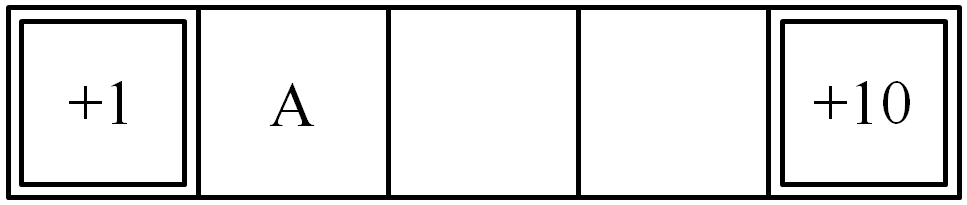
\includegraphics[width=0.4\textwidth]{figures/minigrid-discount.png}
\end{center}

\begin{enumerate}
\item What is the optimal value $V^*(A)$? [4 pts] 
{ \color{red}
10

Since the discount $\gamma=1$ and there are no rewards for any action other than exiting, a policy that simply heads to the right exit state and exits will accrue reward $10$.
This is the optimal policy, since the only alternative reward if $1$, and so the optimal value function has value $10$.
}


\vfill
\item When running value iteration, remember that we start with $V_0(s)=0$ for all $s$.
What is the first iteration $k$ for which $V_k(A)$ will be non-zero? [4 pts]
{\color{red}
2\\
The first reward is accrued when the agent does the following actions (state transitons) in sequence: Left, Exit.
Since two state transitions are necessary before any possible reward, two iterations are necessary for the value function to become non-zero.
}

\vfill

\item What will $V_k(A)$ be when it is first non-zero? [4 pts]
{ \color{red}
1\\
As explained above, the first non-zero value function value will come from exiting out of the left exit cell, which accrues reward $1$.}

\vfill

\item After how many iterations $k$ will we have $V_k(A) = V^*(A)$?  If they will never become equal, write \emph{never}. [4 pts]
{ \color{red}
4\\
The value function will equal the optimal value function when it discovers this sequence of state transitions: Right, Right, Right, Exit.
This will obviously happen in 4 iterations.
}

\vfill

\newpage
Now the situation is as before, but the discount $\gamma$ is less than $1$.
\item If $\gamma = 0.5$, what is the optimal value $V^*(A)$? [4 pts]

{ \color{red}
The optimal policy from A is Right, Right, Right, Exit.
The rewards accrued by these state transitions are: 0, 0, 0, 10.
The discount values are $\gamma^0, \gamma^1, \gamma^2, \gamma^3$, which is $1$, $\frac{1}{2}$, $\frac{1}{4}$, $\frac{1}{8}$.
Therefore, $V^*(A) = 0 + 0 + 0 + \frac{10}{8}$.
}

\vfill

\item For what range of values $\gamma$ of the discount will it be optimal to go \emph{Right} from $A$? [5 pts]

{\color{red}
The best reward accrued with the policy of going left is $\gamma^1 * 1$.
The best reward accrued with the policy of going right is $\gamma^3 * 10$.
We therefore have the inequality $10 \gamma^3 \geq \gamma$, which simplifies to $\gamma \geq \sqrt{1/10}$.
The final answer is $1/\sqrt{10} \le \gamma \le 1$
}

\vfill

\end{enumerate}
